\documentclass{article}
\usepackage{graphicx}
\setlength{\textheight}{9in}
\setlength{\topmargin}{-.5in}
\setlength{\headheight}{0.25in}
\setlength{\headsep}{0.25in}
\setlength{\topskip}{0in}

% arara: pdflatex
\begin{document}

\title{Automated Blocking Posterior Density Plots}
\author{}
\date{}
\maketitle

\begin{figure}[h]
\centerline{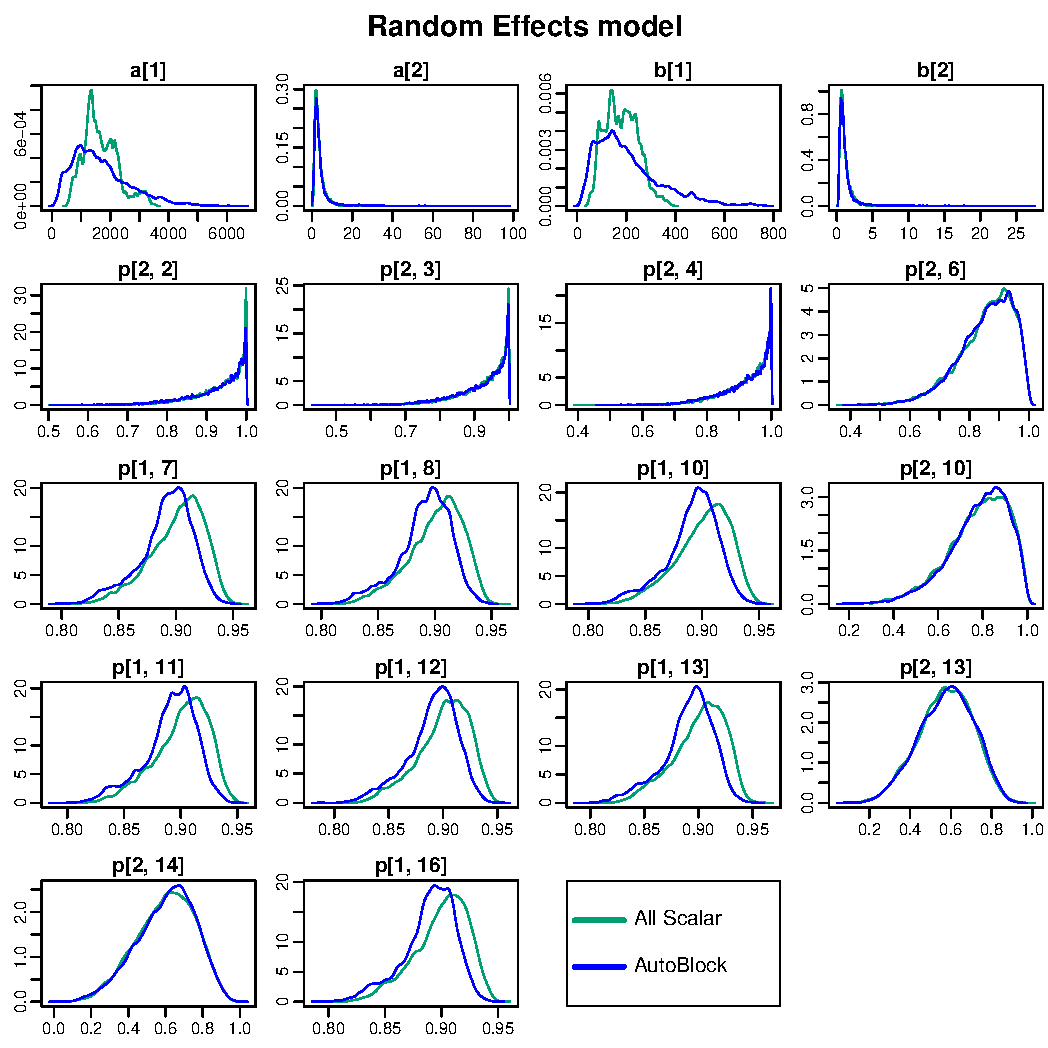
\includegraphics[scale=1.0]{RandomEffectsmodel}}
\end{figure}
\thispagestyle{empty}
\clearpage

\begin{figure}[h]
\centerline{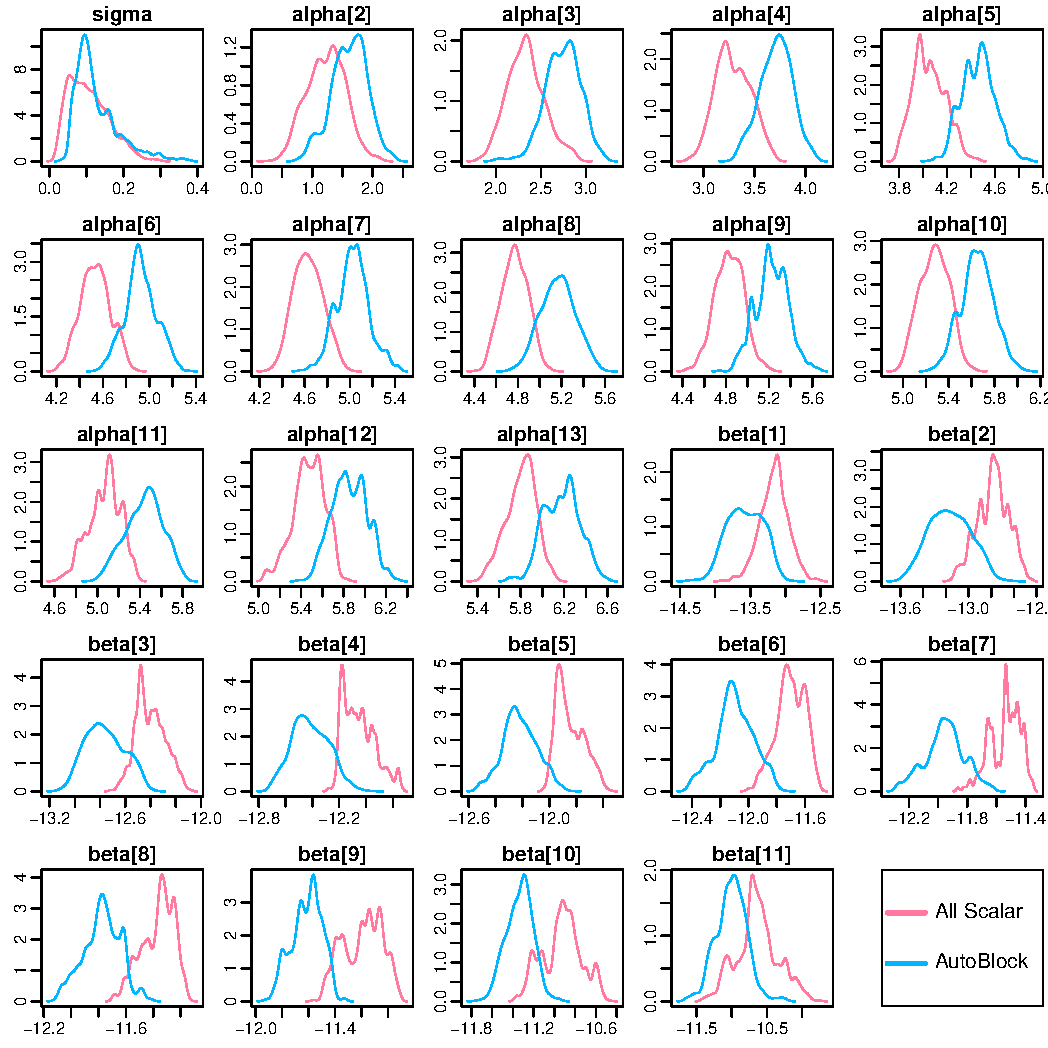
\includegraphics[scale=1.0]{AutoRegressivemodel}}
\end{figure}
\thispagestyle{empty}
\clearpage

\begin{figure}[h]
\centerline{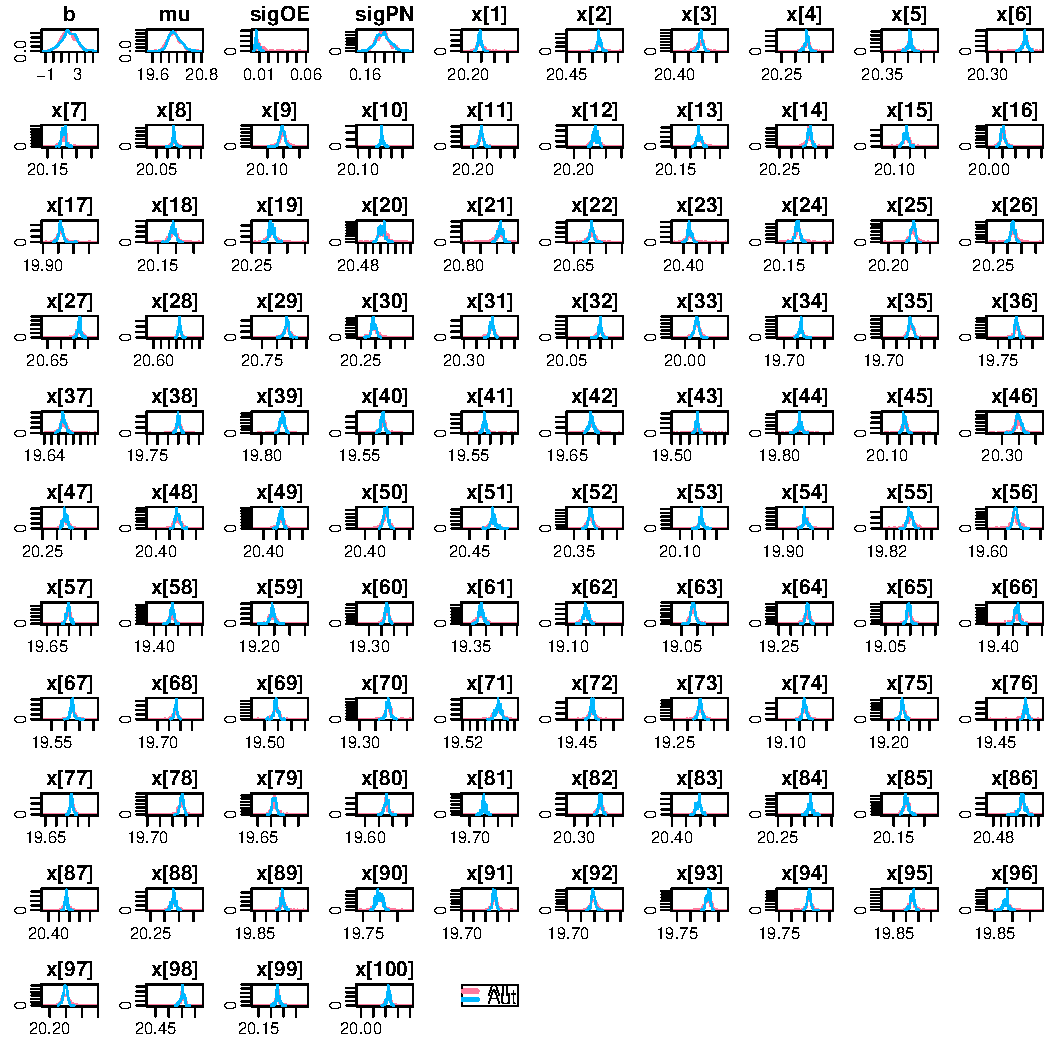
\includegraphics[scale=1.0]{StateSpacemodelindependent}}
\end{figure}
\thispagestyle{empty}
\clearpage

\begin{figure}[h]
\centerline{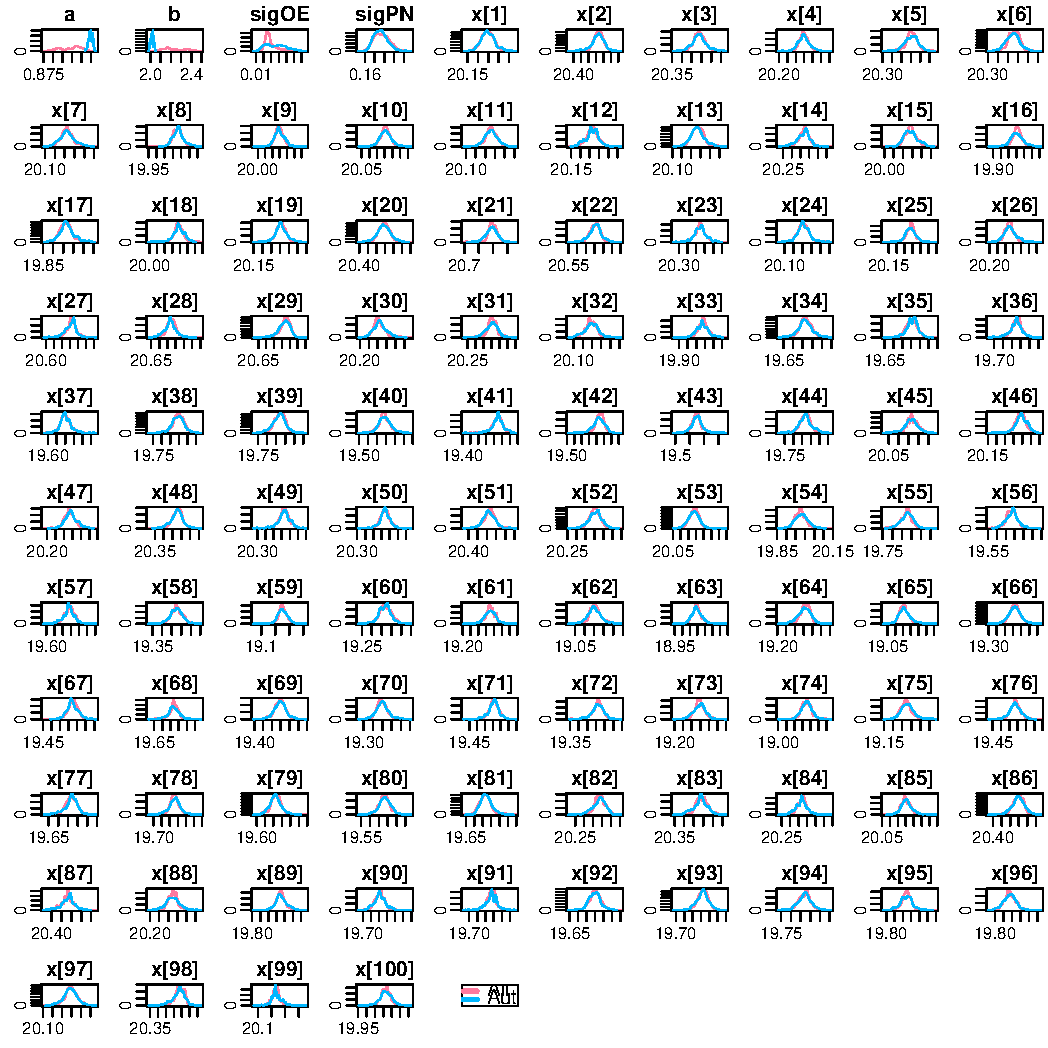
\includegraphics[scale=1.0]{StateSpacemodelcorrelated}}
\end{figure}
\thispagestyle{empty}
\clearpage

\begin{figure}[h]
\centerline{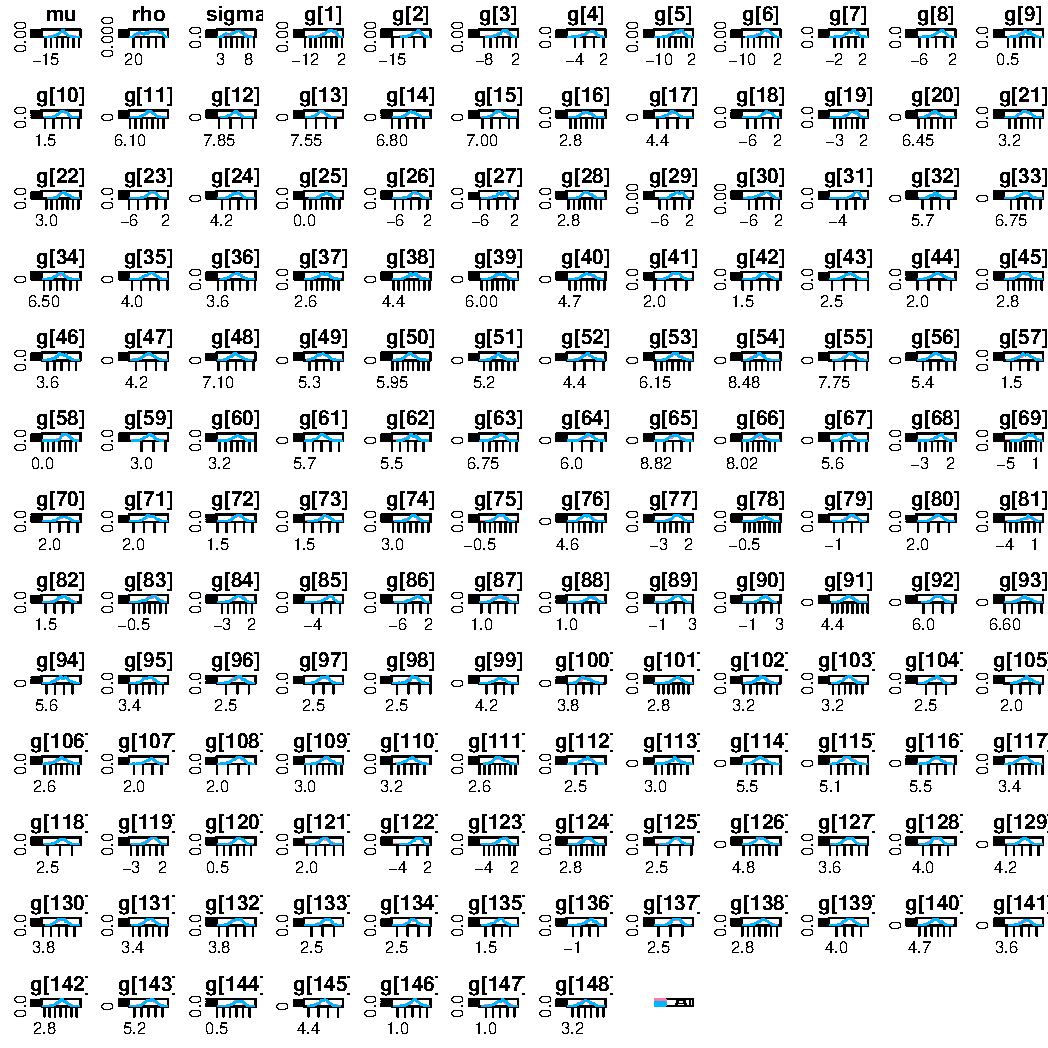
\includegraphics[scale=1.0]{Spatialmodel}}
\end{figure}
\thispagestyle{empty}
\clearpage

\begin{figure}[h]
\centerline{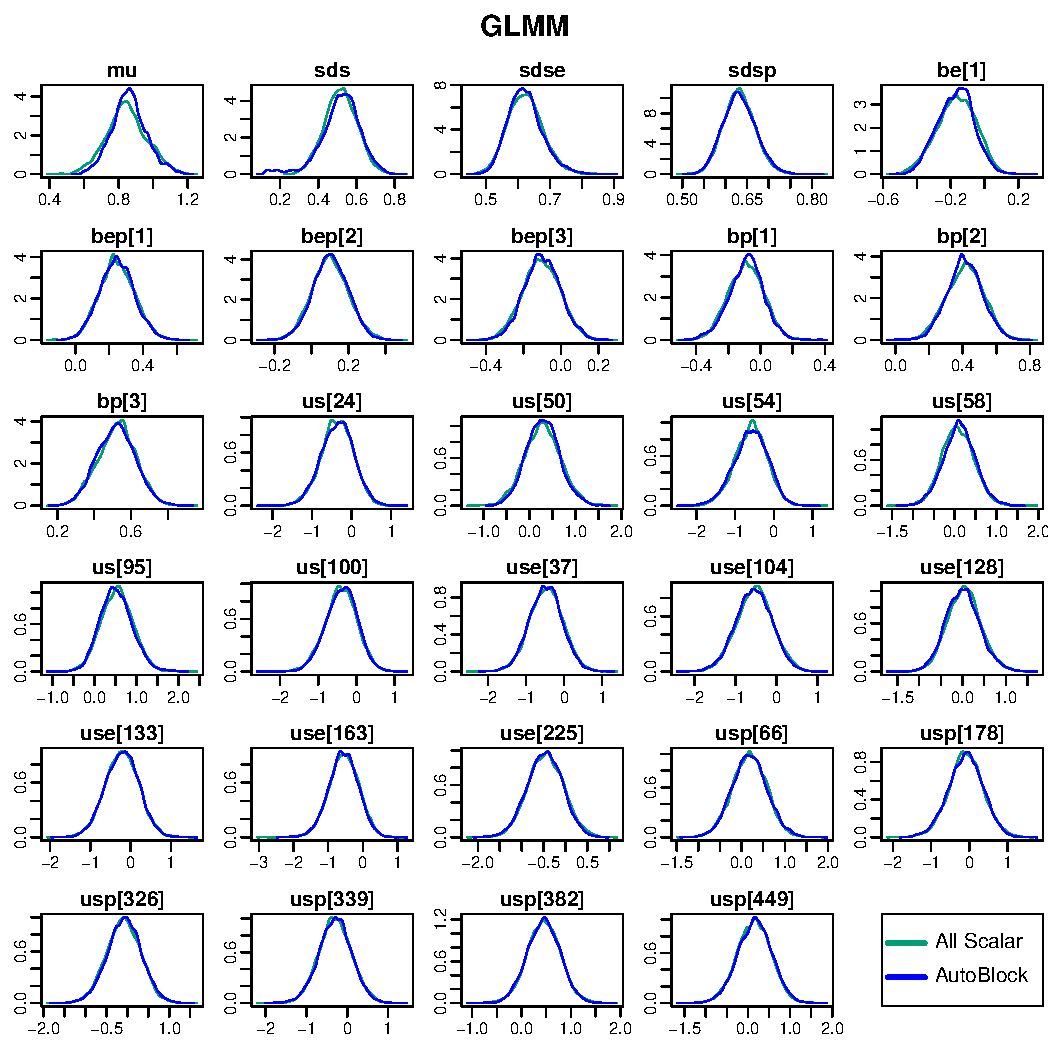
\includegraphics[scale=1.0]{GLMM}}
\end{figure}
\thispagestyle{empty}
\clearpage

\end{document}